\section{Faster R-CNN}  \label{sec:faster_rcnn}

In 2016, the object detection Faster R-CNN model was proposed as an improvement over the Fast R-CNN model. The Faster R-CNN model is composed of two modules . The first module is responsible for generating ROIs with a CNN. The second module is a classification CNN. At its core, Faster R-CNN is a Fast R-CNN model with a region proposal network (RPN) (Figure \ref{fig:faster_rcnn_archite}). Through testing with different datasets like PASCAL VOC and COCO, Fast R-CNN with RPN as a region proposal method consistently achieved higher accuracy scores compared to when generating ROIs with the selective search algorithm. One example is testing the same Fast R-CNN based on VGG-16 on the combined dataset of PASCAL VOC 2007 and 2012, the model with the Selective Search algorithm achieved an mAP score of 70\%, which is not as accurate as when using RPN to generate ROIs at 73.2\% in mAP score \cite{faster_rcnn_2015}.

\begin{figure}[!ht]
    \centering
    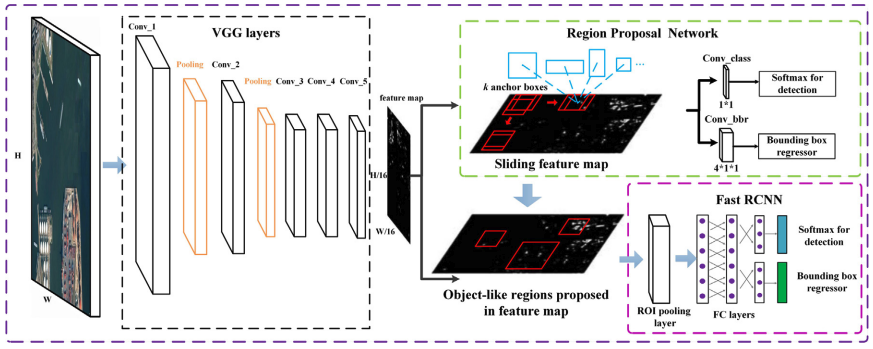
\includegraphics[width=5in]{figures/faster_rcnn_archite.png}
    \caption{Faster R-CNN Overall Architecture \cite{faster_rcnn_architecture_fig}} \label{fig:faster_rcnn_archite}
\end{figure}

The Region Proposal Network (RPN) is a fully connected convolutional network engineered to propose regions of interest (ROIs) regardless of object scales and aspect ratios. RPN accepts any size image as input and outputs several bouding boxes, each with a score representing the possibility of an object residing in the box under consideration. The main advantage of RPN over Selective Search is, while Selective Search is implemented in CPU, RPN is implemented in GPU. Utilizing the computation power of GPU instead of CPU help boost the performance of region proposal tremendously. Moreover, since models like Fast R-CNN also use GPU and convolutional layers to generate detection, RPN can share computation with Fast R-CNN through a multi-task loss. Consequently, reduce the computational power needed for generating ROIs to almost none when added on top of the computation already needed by the object detection module. As a comparison, RPN able to generate ROIs in 0.01 second oppose to 2 seconds with Selective Search, while achieving higher accuracy score overall \cite{faster_rcnn_2015}. Furthermore, unlike Selective Search, which is a fixed algorithm and not trainable, RPN is a learnable neural network. Thus the performance will increase when more data is fed and/or a deeper network is being used. 

The RPN model can be thought of as two stage process. In the first stage, RPN applies a CNN over the inputted image and generates a feature map for the entire image. The same operation is taken in the first stage of Fast R-CNN. Thus, Faster R-CNN can have a CNN to generate the image feature map, and then the image feature map proceeds as input for the second stage of RPN and Fast R-CNN. Thereby sharing computation between the two modules of Faster R-CNN. In the second stage, RPN slides a $3 \times 3$ convolutional layer, then branched to two siblings $1 \times 1$ layers. The first branch is a bounding box regressor that generates a set of four values representing the coordinate of the bounding box. The second branch is a classifier that produces a score for the probability that the object is in the window. At each sliding window location, RPN create an anchor at the center of the window. Then, with 3 different scaling factors and 3 different aspect ratios, RPN generate 9 new proposals with the anchor at the center \ref{fig:faster_rcnn_anchor}. Since RPN behavior is based on the sliding window technique, it exhausted all possible locations, and with the use of 9 different sizes and aspect ratios, RPN gains the translation invariant property. That is, RPN is guaranteed to be able to generate the object's location even if some translation operation is performed on the object.

\begin{figure}[!ht]
    \centering
    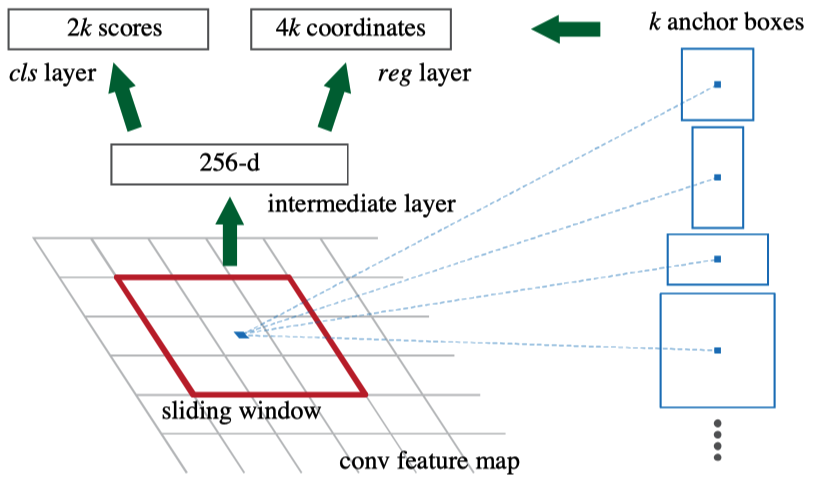
\includegraphics[width=3in]{figures/rpn_anchor.png}
    \caption{Region Proposal Network (RPN) \cite{faster_rcnn_2015}} \label{fig:faster_rcnn_anchor}
\end{figure}

Similar to Fast R-CNN, the RPN model is trained end-to-end with a multi-task loss. The multi-task loss is derived based on the classification loss over two classes (object vs. not object) and the regression loss over two coordinates (predict bounding box vs. truth bounding box), summed across all anchor points. If RPN samples all anchor points, then the model will favor negative false as the majority of RPN's generated box does not overlap with any truth box. To resolve this problem, RPN employs a sample-dropping technique and then randomly selects 256 samples to help balance positive and negative samples \cite{faster_rcnn_2015}. For sample dropping, RPN mark all predicted box with more than 70\% of overlapping with any truth box as positive and any predicted box with less than 30\% of overlapping with any truth box as negative, then drop any predicted box that is neither classified as positive nor negative. With that being said, the RPN training process consists of 3 steps. In the first step, the model initialized the share CNN with a pre-trained model like VGG-16 and randomly assigned weight values for the newly added layer in RPN. Then RPN is trained with the stochastic gradient descent (SGD) method, where each mini-batch consists of 256 samples that either overlap more than 70\% or less than 30\%. At each iteration, the model uses the multi-task loss as described previously to perform backpropagation.

With the understanding of end-to-end training for RPN and Fast R-CNN, we can now train the two components of Faster R-CNN independently. However, when training RPN and Fast R-CNN separately, optimizing the shared convolutional layers for the object proposal task does not guarantee that these layers will be optimized for the classification task because the network learns significantly differently for the two tasks. To address this issue, Faster R-CNN employs a four-step alternative training procedure. Faster R-CNN trains an RPN model separately in the first phase as described previously. Faster R-CNN trained a separate Fast R-CNN network in the second phase, which uses the ROIs generated by RPN in the first step as input for the classification task. Once the second phase is completed, Faster R-CNN trains the unique layer to RPN using the trained Fast R-CNN. This means that all Fast R-CNN layers are being fixed during this step, while the $3 times 3$ convolutional layer and two siblings $1 times 1$ layers unique to RPN are being trained. In the last phase, Faster R-CNN fixed the shared convolutional layers and layers specific to the RPN, so training occurs on Fast R-CNN's unique layers. This 4-step alternative training process is carried through each minibatch of SGD. The author of Faster R-CNN mentions two other shared schemes, approximate joint training, and non-approximate joint training, in addition to the alternative training scheme \cite{faster_rcnn_2015}. Unfortunately, both methods are impeded by issues beyond this study's scope; therefore, we will not go into depth.
